\documentclass[25pt, a0paper, portrait,innermargin=35mm,
blockverticalspace=30mm, colspace=90mm, subcolspace=3mm]{tikzposter}
% font size: The size of the text in the main body may be set as : 12pt, 14pt, 17pt, 20pt, or 25pt;
% paper size: Currently, paper sizes may be set to : a0paper, a1paper, or a2paper;
% orientation: Either landscape or portrait
\usepackage[utf8]{inputenc}
\usepackage[T1]{fontenc}

\usepackage[ngerman]{babel}
\usepackage{pdfpages}
\usepackage{tikzpagenodes}

\usepackage{rustic}
\usepackage{lmodern}
%\usepackage[sfdefault,lf]{carlito}
\usepackage{fontawesome}
\usepackage{blindtext}
\usepackage{comment}
\usepackage{hyperref}
\usepackage{listings}

\usetheme{Simple}
%\usetitlestyle{Empty}\usebackgroundstyle{Empty}

%--------------------------------------
\usepackage[light,default]{raleway}

%-------------- FARBEN

\usepackage[usenames, dvipsnames]{color} % um diese Color-Names zu verwenden: https://de.sharelatex.com/learn/Using_colours_in_LaTeX#!#Reference_guide z.B. \color{RubineRed}

\definecolor{AlchemicalLilac}{HTML}{6E0D98} %#660022
\definecolor{GamsGreen}{HTML}{37980D} %6F906E
\definecolor{AlchemyBlue}{HTML}{0D089F} %6F906E
\definecolor{AlchemyRed}{HTML}{98290D} %6F906E
\definecolor{MaierPage}{HTML}{d7c8a8}

\colorlet{AlchemicalLilac}{AlchemicalLilac!90} % Farben etwas heller machen
\colorlet{GamsGreen}{GamsGreen!90}


\definecolor{LightAlchemicalLilac}{RGB}{152,51,85} %#A3244E

%---------------- bei den Farben gibt es immer bg und fg, wobei bg Hintergrund und fg normalerweise Schriftfarbe ist. Dies ist zu definieren für backgroundcolor, framecolor, dann für titlefg/bgcolor, selbiges für (inner)blocktitle und blockbody, und ggf. für notefg/bgcolor
\colorlet{backgroundcolor}{MaierPage}  % warum geht das nicht?!
\colorlet{titlebgcolor}{AlchemicalLilac}
\colorlet{titlefgcolor}{GamsGreen}
\colorlet{blocktitlefgcolor}{AlchemicalLilac}

% \colorlet{backgroundcolor}{MaierPage}


\usepackage{sarah-commands}


\begin{document}


\draw[fill=AlchemicalLilac,draw=AlchemicalLilac,minimum width=\paperwidth](header) (-45cm,60cm) -- ++(0,-50cm) -- (\paperwidth+20cm,60cm) --  ++(0,0);
\node[outer sep=2cm,align=center] at (0cm,48cm) {
\begin{minipage}{\textwidth}
\begin{minipage}{0.25\textwidth}
%\vspace{13cm}\hspace{4cm}
\includegraphics[width=\textwidth]{maierus.png}

\end{minipage}\hfill
% --------------- TITLE
% -------------------------------------------------------------------------------
\begin{minipage}{0.5\textwidth} % TODO!
\vspace{3cm}
\color{GamsGreen}\fontsize{110pt}{110pt}\selectfont 
\textbf{POÉSIE}AL\textbf{CHIMIQUE}\\[0.5em]
\color{white}\fontsize{45pt}{45pt}\selectfont Comment \textbf{approcher} le \textbf{langage} de \textbf{l’alchimie} \\ néo-\textbf{latine} du \textbf{17ème} siècle\\à travers un \textbf{thesaurus} \\ Semantic \textbf{Web}? \\
\end{minipage}\hspace{3cm}
\end{minipage}

};


% --------------- Maier-Bild
% -------------------------------------------------------------------------------
\draw[fill=MaierPage,draw=MaierPage](maierinfo) (-18,45) circle (9);
\node[align=left] at (-16,49) {\Large\textbf{Michael Maier} \\ 1568--1622};
\node[align=left] at (-15,45) {auteur de traités \\alchimiques};
\node[align=left] at (-14,41) {\footnotesize{}\emph{Atalante fugitive} (1617)\\ \footnotesize\emph{Viatorium} (1618) \\ \dots };

\draw[fill=MaierPage] (19,5) circle (13cm);
\node[above left=16cm] at(TP@title.south) {
\includegraphics[width=0.3\textwidth]{maierus}};


% --------------- TITLE
% -------------------------------------------------------------------------------
\begin{columns}
\column{0.55}
\block{}
{
\vspace{-14cm}
\begin{minipage}{0.05\textwidth}
\color{white}.
\end{minipage}\hfill
\begin{minipage}{0.4\textwidth}
\subsection*{\Large Le problème}
La méthode de communication alchimique est l’analogie. 
Les textes alchimiques utilitsent des outils de codage:
\begin{enumerate}
    \item \textbf{Dispersion de la science} Le savoir est divisé entre plusieurs texts.
    \item \textbf{\emph{Decknamen}} Mots symboles, communication par analogies, néologismes fréquents, sens non-stable.
\end{enumerate}


\subsection*{\Large Solution I:}
Thesaurus des \emph{Decknamen}:
\begin{enumerate}
    \item trouver les \emph{Decknamen} du thésaurus dans le texte
    \item générer le ``KWIC'' des \emph{Decknamen}: non-linguistique, montrant les \emph{Decknamen} proches
    \item retrouver d'autres Decknamen dans le KWIC
    \item classifier les contexts des \emph{Decknamen}: héros mythologiques, parler sur l'Opus Magnum, etc.
    \item comparer chaque occurence avec l'impression générale: usage nouveau ou suivant le modèle, etc.

\end{enumerate}
\end{minipage}\hfill


%\draw[fill=AlchemyRed,draw=AlchemyRed] (0,0) circle (5);\draw[fill=GamsGreen,draw=GamsGreen] (0,10) circle (5);
%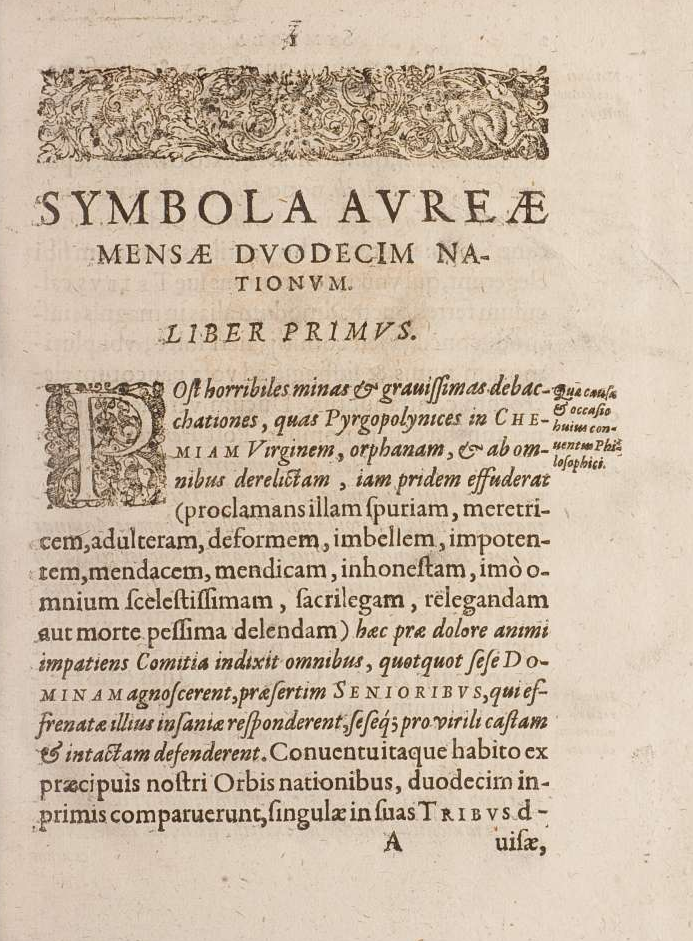
\includegraphics[width=0.2\textwidth]{symbola.png}
}

\column{0.370}
\block{}
{
\vspace{-25cm}
\hspace{3cm}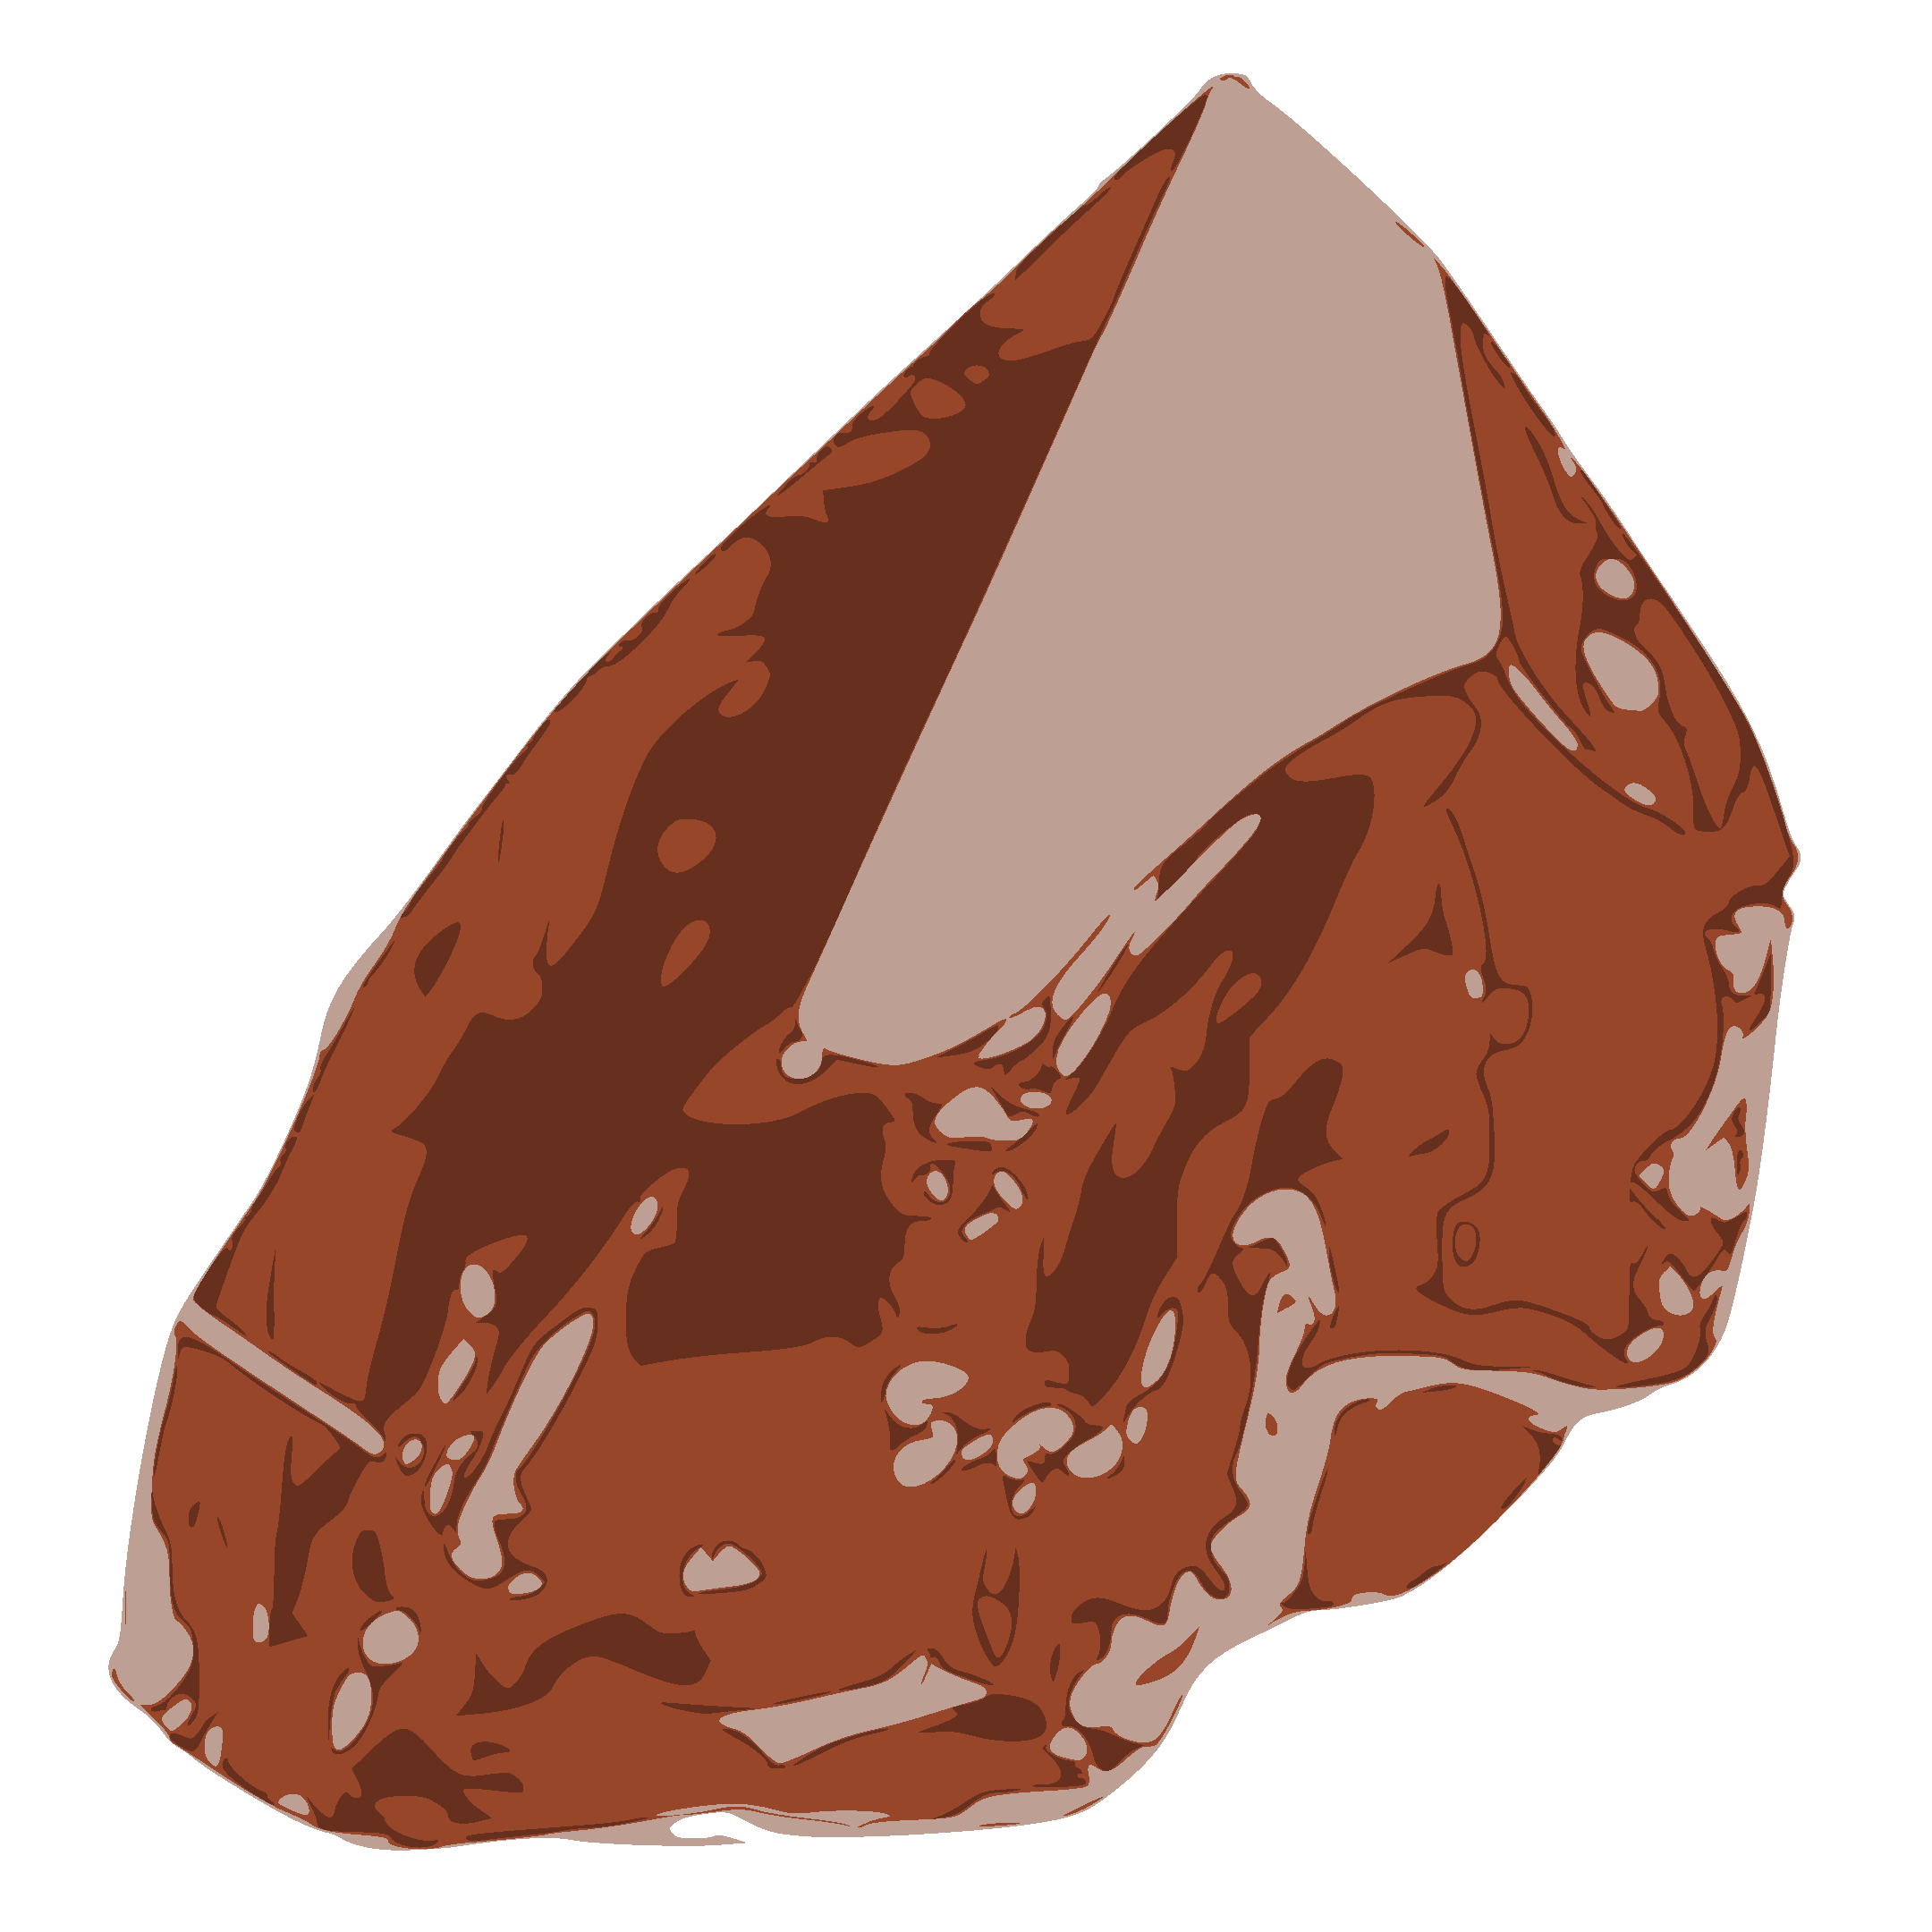
\includegraphics[width=0.2\textwidth]{steindweisen-bg.png}

{\bf\large Solution II: Associations en RDFS}

:PhilosophersStone :hasColor :red. \\
:red :hasChemicalProperty :tingiert. (\emph{teinte}) \\
:tingiert :givesPhysicalProperty :citrinitas. \\
:Gold :hasColor :citrinitas.\\[1em]

$\to$ génération d'associations \\ \phantom{xxxx} entre les concepts

}

\end{columns}
\begin{columns}
 \column{0.82}
    \block{}{
 \vspace{-1cm}   
\coloredbox[width=0.82\textwidth,bgcolor=GamsGreen!10,fgcolor=AlchemicalLilac,framecolor=GamsGreen!10]{

\begin{minipage}[t]{0.12\textwidth}
\hspace{2cm} 
\includegraphics[width=0.8\textwidth]{hermes-viatorium2.png} \hspace{2cm} 

\end{minipage}\hfill
\begin{minipage}[t]{0.69\textwidth}

\subsection*{\Large Exemple:}
\lstinputlisting{example-ulysses.xml}
 $\to$ context:metals, context:planets, context:mythological, context:alchemicalWorkMeta

\begin{itemize}
    \item Isis, Osiris, Vulcanus, heros $\to$ alchemicalInnovators
    \item Chymici, artificis $\to$ alchemicalWork (meta)
    \item Aegyptus, Trismegistos $\to$ alchemicalTradition
    \item Hydrargyrum, sol, plumbum $\to$ planets, metals
\end{itemize}

\lstinputlisting{example-mercurius.xml}


 $\to$ context:mythological, context:alchemicalWorkMeta
 
\begin{itemize}
    \item Homer, Troia, grecs de la mythologie  $\to$  context:mythological
    \item Heroes, persona, artifex, labor manuum, ars philosophica, Chymicos, Chemia  $\to$  context:alchemicalWork (meta)
\end{itemize}

\end{minipage}\hfill

} 
}
    
    \column{0.15}
        \block{}{
\vspace{-16cm}
\hspace{-13cm}\bubblediagram{{\color{white}\textbf{Méthode}},  NLP, \textbf{Annotation}, {thésaurus},Semantic\\ Web,{SKOS-XL}, RDFS, \textbf{TEI}}
		
		%\bubbleicon{\Huge\faBook}{Reading}{white}{\huge}
 }
    
\end{columns}


\draw[fill=AlchemicalLilac,draw=AlchemicalLilac,minimum width=\paperwidth] (-45cm,-51cm) -- ++(0,7cm) -- (\paperwidth,-51cm) --  cycle;


\node [above right,outer sep=0pt,minimum width=\paperwidth,minimum height=5cm,align=center,draw=AlchemicalLilac,fill=AlchemicalLilac](footer) at (bottomleft) {
\begin{minipage}{\textwidth}
\vspace{1cm}\hspace{2cm}\color{white}\Large\MakeUppercase{Sarah\textbf{Lang}}\hspace{0.5cm} \protect\url{sarah.lang@uni-graz.at}\hfill

\includegraphics[width=0.07\textwidth]{gamsweiss.png}\hspace{2cm}

\includegraphics[width=0.07\textwidth]{ZIM_weiss.png}\hspace{2em}

\includegraphics[width=0.07\textwidth]{kfFarbe.jpg}\hspace{2em}\vspace{2cm}
\end{minipage}
};

\end{document}
